\documentclass[twocolumn,10pt,journal]{IEEEtran}
\usepackage[utf8]{inputenc}
\usepackage[spanish]{babel}
\usepackage{amsmath}
\usepackage{amssymb}
\usepackage{graphicx}
\usepackage{booktabs}
\usepackage{hyperref}
\usepackage{microtype}
\usepackage{cite}

\title{Análisis de Complejidad Computacional y Escalamiento Empírico de Clasificadores en la Auditoría de Sesgo de Alineación en Modelos de Lenguaje Grande}

\author{Entregable del Proyecto Integrador --- Área de Complejidad Algorítmica}

\markboth{Complejidad Computacional, Mayo de 2026}{Estudio de Complejidad Computacional}

\begin{document}
\maketitle
\begin{abstract}
Este reporte presenta un analisis de la complejidad asintótica (Big O) y el comportamiento de dos modelos de clasificacion de Aprendizaje Supervisado (Machine learning); K-Nearest Neighbors (KNN) con similitud coseno y Regresión Logistica con descendso de gradiente, aplicados al problema de auditoria de sesgo de alineacion (aligment) en LLMs. Utilizando el dataset extraido de ShareChat, se implemantaron ambos algoritmos de ML “desde cero”, con una implementacion manual, comparando su rendimiento en contra de soluciones optimizadas de la biblioteca scikit-learn. Los resultados demuestran las limitaciones del modelado manual bajo grandes volumenes de datos.
\end{abstract}

\begin{IEEEkeywords}
Complejidad Algorítmica, Cota Asintótica, Big-O, K-Nearest Neighbors, Regresión Logística, Sesgo de Alineación, Similitud Coseno, Descenso de Gradiente.
\end{IEEEkeywords}

\section{Introducción}

\IEEEPARstart{L}{a} llegada de los Modelos Grandes de Lenguaje (LLMs) revolucionó el procesamiento de lenguaje natural (NLP). Sin embargo, olas de investigación enfocadas en garantizar que estas herramientas respondan bajo estándares seguros y alineados (\textit{AI Safety}) han puesto a la teoría de la alineación como prioridad crítica dentro de la investigación por la seguridad de la IA. El estudio de la hipótesis del \textit{Sesgo de Alineación} evalúa si los modelos comerciales y de código abierto rechazan adecuadamente el contenido hostil en diferentes lenguas y plataformas \cite{ouyang2022}.

Para predecir el comportamiento de seguridad ante prompts tóxicos basándonos en atributos de entrada (longitud de prompts, plataforma e idioma) se hace indispensable la implementación de modelos de clasificación como KNN y Regresión Logística. En este contexto, no solo importa la precisión del clasificador, sino también su eficiencia computacional. 

El presente reporte tiene como finalidad formalizar matemáticamente los dos algoritmos implementados de manera manual en el proyecto, presentar de forma científica las complejidades asintóticas utilizando la notación formal Big-O \cite{knuth1976}, y comparar sus curvas de escalamiento en tiempo ($T(N)$) contra las implementaciones optimizadas de la librería sklearn.

\section{Metodología Matemática de los Algoritmos}

Para la elaboración del proceso del proyecto, implementamos de forma manual dos modelos estándar de aprendizaje supervisado. Estos modelos trabajan con el texto transformado en 'vectores dispersos' mediante el método TF-IDF, dentro de un espacio de características de dimensión $d$.

\subsection{K-Nearest Neighbors (KNN) con Similitud Coseno}
El clasificador KNN es un método sencillo y no paramétrico de aprendizaje basado en instancias o perezoso (\textit{lazy learning}) \cite{hastie2009}. Este modelo no tiene una fase de entrenamiento formal; en su lugar, simplemente almacena los datos de entrenamiento $\mathbf{X}_{\text{train}} \in \mathbb{R}^{N \times d}$. 

Para clasificar un nuevo dato o prompt de consulta $\mathbf{q} \in \mathbb{R}^d$, el algoritmo calcula qué tan parecido es $\mathbf{q}$ con cada ejemplo $\mathbf{x}_i$ ($i = 1, \dots, N$) usando la \textit{Similitud Coseno}, la cual se define matemáticamente como:
\begin{equation}
\text{sim}(\mathbf{q}, \mathbf{x}_i) = \frac{\mathbf{q} \cdot \mathbf{x}_i}{\|\mathbf{q}\|_2 \|\mathbf{x}_i\|_2} = \frac{\sum_{j=1}^d q_j x_{i,j}}{\sqrt{\sum_{j=1}^d q_j^2} \sqrt{\sum_{j=1}^d x_{i,j}^2}}
\end{equation}

A partir de esto, calculamos la \textit{Distancia Coseno} para medir la separación:
\begin{equation}
d_{\text{cos}}(\mathbf{q}, \mathbf{x}_i) = 1 - \text{sim}(\mathbf{q}, \mathbf{x}_i)
\end{equation}

Luego, buscamos el conjunto $\mathcal{N}_K(\mathbf{q})$ con las $K$ muestras de entrenamiento que tengan la menor distancia $d_{\text{cos}}$ con respecto a $\mathbf{q}$. Finalmente, predecimos la clase $\hat{y}$ tomando la etiqueta más común (votación mayoritaria):
\begin{equation}
\hat{y} = \text{mode} \left( \{ y_i \mid \mathbf{x}_i \in \mathcal{N}_K(\mathbf{q}) \} \right)
\end{equation}

El pseudocódigo completo de nuestra implementación manual de este algoritmo se describe en la Tabla I.

\begin{table}[h]
\centering
\caption{Pseudocódigo del Clasificador KNN Manual}
\label{alg:knn}
\begin{tabular}{p{8cm}}
\toprule
\textbf{Algoritmo 1:} KNN con Similitud Coseno \\
\midrule
\textbf{Entrada:} Punto de consulta $\mathbf{q} \in \mathbb{R}^d$, matriz de entrenamiento $\mathbf{X} \in \mathbb{R}^{N \times d}$, etiquetas $\mathbf{y} \in \{0, 1\}^N$, número de vecinos $K$. \\
\textbf{Salida:} Etiqueta predicha $\hat{y} \in \{0, 1\}$. \\
\midrule
1: \textbf{Procedimiento} \textsc{PredecirKNN}($\mathbf{q}, \mathbf{X}, \mathbf{y}, K$) \\
2: \quad Inicializar vector de similitudes $\mathbf{s} \in \mathbb{R}^N$ \\
3: \quad \textbf{Para} $i = 1$ \textbf{hasta} $N$ \textbf{hacer} \\
4: \quad \quad $\mathbf{s}_i \leftarrow \frac{\mathbf{q} \cdot \mathbf{x}_i}{\|\mathbf{q}\|_2 \|\mathbf{x}_i\|_2 + \epsilon}$ \hfill $\triangleright$ Similitud Coseno \\
5: \quad \textbf{Fin Para} \\
6: \quad $\mathcal{I}_K \leftarrow \text{obtener\_indices\_top\_K}(\mathbf{s})$ \hfill $\triangleright$ Índices de las $K$ mayores similitudes \\
7: \quad $\mathbf{y}_K \leftarrow \{ \mathbf{y}_j \mid j \in \mathcal{I}_K \}$ \hfill $\triangleright$ Etiquetas de los $K$ vecinos \\
8: \quad $\hat{y} \leftarrow \text{moda}(\mathbf{y}_K)$ \hfill $\triangleright$ Votación mayoritaria \\
9: \quad \textbf{Retornar} $\hat{y}$ \\
\bottomrule
\end{tabular}
\end{table}

\subsubsection{Cálculo Detallado en Librerías Utilizadas (KNN)}
Para programar la similitud coseno de forma manual en Python, usamos la biblioteca \texttt{numpy} con las siguientes funciones:
\begin{itemize}
    \item \textbf{np.dot(sample, X.T)}: Realiza el producto punto matricial entre el vector de prueba y los de entrenamiento. En segundo plano (usando librerías BLAS optimizadas), calcula la suma $\sum_{j=1}^d q_j X_{i,j}$ para cada elemento $i$.
    \item \textbf{np.linalg.norm(X, axis=1)}: Obtiene la norma de cada vector $\|\mathbf{x}_i\|_2 = \sqrt{\sum_{j=1}^d X_{i,j}^2}$ para poder normalizar las distancias.
\end{itemize}
Por otro lado, la versión optimizada de \texttt{scikit-learn} tiene implementaciones más eficientes para buscar vecinos rápidamente:
\begin{itemize}
    \item \textbf{KD-Tree}: Es una estructura de árbol que divide el espacio de datos de tamaño $N \times d$ usando hiperplanos. Cuando se busca un vecino, el algoritmo calcula la distancia a las fronteras del árbol y evita calcular la distancia con datos que están muy lejos (poda del árbol). Esto permite reducir el costo de buscar vecinos de un orden lineal $\mathcal{O}(N)$ a uno logarítmico $\mathcal{O}(\log N)$ en casos ideales.
\end{itemize}

\subsection{Regresión Logística con Descenso de Gradiente}
La Regresión Logística es un modelo de clasificación muy utilizado \cite{hastie2009}. En este algoritmo, la probabilidad de que un texto o prompt $\mathbf{x} \in \mathbb{R}^d$ sea clasificado en la categoría de interés ($y = 1$) se calcula con la función sigmoide:
\begin{equation}
h_{\mathbf{w}, b}(\mathbf{x}) = \sigma(\mathbf{w}^T \mathbf{x} + b) = \frac{1}{1 + e^{-(\mathbf{w}^T \mathbf{x} + b)}}
\end{equation}
donde $\mathbf{w} \in \mathbb{R}^d$ son los pesos del modelo y $b \in \mathbb{R}$ es el sesgo o término independiente.

Para entrenar este modelo, buscamos los mejores valores de $\mathbf{w}$ y $b$ minimizando la función de costo conocida como Entropía Cruzada Binaria. En nuestra implementación manual no usamos penalización ($\lambda = 0$), pero en las librerías profesionales se suele agregar un término de regularización $L_2$ para evitar que el modelo se sobreajuste a los datos:
\begin{equation}
J(\mathbf{w}, b) = -\frac{1}{N} \sum_{i=1}^N \left[ y^{(i)} \ln(h^{(i)}) + (1-y^{(i)}) \ln(1-h^{(i)}) \right] + \frac{\lambda}{2N} \|\mathbf{w}\|_2^2
\end{equation}
donde $h^{(i)} = h_{\mathbf{w}, b}(\mathbf{x}^{(i)})$ y $\lambda$ es el parámetro que controla la fuerza de la regularización.

Para encontrar el mínimo de esta función, implementamos el algoritmo de Descenso de Gradiente. Las derivadas de la función de costo con respecto a los parámetros (gradientes) se calculan como:
\begin{equation}
\frac{\partial J}{\partial \mathbf{w}} = \frac{1}{N} \mathbf{X}^T (\mathbf{h} - \mathbf{y}) + \frac{\lambda}{N} \mathbf{w}
\end{equation}
\begin{equation}
\frac{\partial J}{\partial b} = \frac{1}{N} \sum_{i=1}^N (h^{(i)} - y^{(i)})
\end{equation}

En cada iteración de entrenamiento $t$, actualizamos los pesos y el sesgo usando una tasa de aprendizaje $\alpha$:
\begin{equation}
\mathbf{w}^{(t+1)} \leftarrow \mathbf{w}^{(t)} - \alpha \frac{\partial J}{\partial \mathbf{w}}
\end{equation}
\begin{equation}
b^{(t+1)} \leftarrow b^{(t)} - \alpha \frac{\partial J}{\partial b}
\end{equation}

El flujo paso a paso de este entrenamiento manual se detalla en el pseudocódigo de la Tabla II.

\begin{table}[h]
\centering
\caption{Pseudocódigo del Entrenamiento de Regresión Logística}
\label{alg:logreg}
\begin{tabular}{p{8cm}}
\toprule
\textbf{Algoritmo 2:} Regresión Logística por Descenso de Gradiente \\
\midrule
\textbf{Entrada:} Matriz de características $\mathbf{X} \in \mathbb{R}^{N \times d}$, etiquetas reales $\mathbf{y} \in \{0, 1\}^N$, tasa de aprendizaje $\alpha$, número de iteraciones $T$. \\
\textbf{Salida:} Vector de pesos ajustados $\mathbf{w} \in \mathbb{R}^d$ y sesgo $b \in \mathbb{R}$. \\
\midrule
1: \textbf{Procedimiento} \textsc{EntrenarRegresionLogistica}($\mathbf{X}, \mathbf{y}, \alpha, T$) \\
2: \quad Inicializar $\mathbf{w} \leftarrow \mathbf{0} \in \mathbb{R}^d$ y $b \leftarrow 0$ \\
3: \quad \textbf{Para} $t = 1$ \textbf{hasta} $T$ \textbf{hacer} \\
4: \quad \quad $\mathbf{z} \leftarrow \mathbf{X} \mathbf{w} + b$ \hfill $\triangleright$ Combinación lineal \\
5: \quad \quad $\mathbf{h} \leftarrow \frac{1}{1 + e^{-\mathbf{z}}}$ \hfill $\triangleright$ Predicción probabilística (Sigmoide) \\
6: \quad \quad $\mathbf{h} \leftarrow \text{clip}(\mathbf{h}, 10^{-15}, 1 - 10^{-15})$ \hfill $\triangleright$ Estabilidad numérica \\
7: \quad \quad $\mathbf{g}_{\mathbf{w}} \leftarrow \frac{1}{N} \mathbf{X}^T (\mathbf{h} - \mathbf{y})$ \hfill $\triangleright$ Gradiente de los pesos ($\lambda=0$) \\
8: \quad \quad $g_b \leftarrow \frac{1}{N} \sum_{i=1}^N (\mathbf{h}_i - \mathbf{y}_i)$ \hfill $\triangleright$ Gradiente del sesgo \\
9: \quad \quad $\mathbf{w} \leftarrow \mathbf{w} - \alpha \, \mathbf{g}_{\mathbf{w}}$ \hfill $\triangleright$ Actualización de pesos \\
10: \quad \quad $b \leftarrow b - \alpha \, g_b$ \hfill $\triangleright$ Actualización de sesgo \\
11: \quad \textbf{Fin Para} \\
12: \quad \textbf{Retornar} $\mathbf{w}, b$ \\
\bottomrule
\end{tabular}
\end{table}

\subsubsection{Cálculo Detallado en Librerías Utilizadas (Regresión Logística)}
Para la regresión logística hecha a mano, usamos las siguientes herramientas de la librería \texttt{numpy}:
\begin{itemize}
    \item \textbf{np.exp(-z)}: Calcula el valor de $e^{-z_i}$ para cada dato. Internamente, el procesador evalúa esto usando aproximaciones matemáticas muy eficientes a nivel de hardware.
    \item \textbf{np.clip(z, -250, 250)}: Esta función limita los valores de $\mathbf{z}$ para que estén dentro del rango $[-250, 250]$. Hacemos esto para evitar errores de desbordamiento numérico (\textit{overflow/underflow}), ya que si calculamos el exponencial de números muy grandes, Python puede producir valores infinitos o indeterminados (\texttt{NaN}).
\end{itemize}
En comparación, la librería \texttt{scikit-learn} utiliza un optimizador más avanzado:
\begin{itemize}
    \item \textbf{L-BFGS}: Es un método numérico de optimización de segundo orden que pertenece a la familia cuasi-Newton. En lugar de usar solo la dirección del gradiente, este optimizador estima la curvatura de la función usando información de las segundas derivadas (aproximación de la matriz Hessiana). Lo hace guardando únicamente un historial de los últimos $m$ cambios de pesos y gradientes en memoria (donde $m$ suele ser pequeño, como $10$), evitando guardar matrices gigantescas. Esto permite que el modelo encuentre el punto óptimo muchísimo más rápido que el descenso de gradiente estándar.
\end{itemize}

\section{Análisis de Complejidad Computacional Asintótica (Big-O)}

\begin{table*}[t]
\centering
\caption{Resumen comparativo de Complejidad Asintótica (Big-O)}
\label{tab:complexity}
\begin{tabular}{@{}lllll@{}}
\toprule
\textbf{Algoritmo} & \textbf{Fase de Entrenamiento (Tiempo)} & \textbf{Fase de Predicción (Tiempo)} & \textbf{Complejidad Espacial (Memoria)} \\ \midrule
\textbf{KNN Manual} & $\mathcal{O}(1)$ & $\mathcal{O}(M \cdot (N \cdot d + N \log K))$ & $\mathcal{O}(N \cdot d)$ \\
\textbf{KNN Scikit-Learn (Brute)} & $\mathcal{O}(1)$ & $\mathcal{O}(M \cdot N \cdot d)$ (optimizado a nivel BLAS) & $\mathcal{O}(N \cdot d)$ \\
\textbf{KNN Scikit-Learn (KD-Tree)} & $\mathcal{O}(N \cdot d \log N)$ & $\mathcal{O}(M \cdot d \log N)$ (para $d \ll N$) & $\mathcal{O}(N \cdot d)$ \\
\midrule
\textbf{Reg. Logística Manual (GD)} & $\mathcal{O}(T \cdot N \cdot d)$ & $\mathcal{O}(M \cdot d)$ & $\mathcal{O}(d)$ \\
\textbf{Reg. Logística Scikit (L-BFGS)} & $\mathcal{O}(T' \cdot m \cdot d)$ (donde $T' \ll T$, $m \approx 10$) & $\mathcal{O}(M \cdot d)$ & $\mathcal{O}(m \cdot d)$ \\
\bottomrule
\end{tabular}
\end{table>

En esta sección, calculamos las complejidades asintóticas teóricas (Big-O) de las implementaciones manuales y las comparamos con las de \texttt{scikit-learn} \cite{pedregosa2011}. Para este análisis, definimos las siguientes variables: $N$ es la cantidad de ejemplos en el conjunto de entrenamiento, $M$ es el número de ejemplos nuevos que queremos predecir, $d$ es la dimensión de los vectores de características (donde $d = 1000$ debido a los términos obtenidos en TF-IDF), $K$ representa el número de vecinos elegidos para KNN, y $T$ es el total de iteraciones en el descenso de gradiente.

\subsection{Complejidad Teórica de KNN}

\subsubsection{Fase de Entrenamiento}
Como el algoritmo KNN manual es un método basado en instancias, no realiza ningún cálculo durante la fase de entrenamiento; simplemente guarda en la memoria la matriz de características y las etiquetas correspondientes. Por lo tanto, el tiempo de entrenamiento es constante:
\begin{equation}
T_{\text{train}}^{\text{manual}}(N, d) = \mathcal{O}(1)
\end{equation}
Por su parte, el espacio en memoria (complejidad espacial) necesario para guardar estos datos depende directamente del tamaño de la entrada:
\begin{equation}
S_{\text{train}}^{\text{manual}}(N, d) = \mathcal{O}(N \cdot d)
\end{equation}

\subsubsection{Fase de Predicción}
Para clasificar un conjunto de $M$ nuevos ejemplos $\mathbf{q}$, el algoritmo debe realizar dos pasos principales por cada uno de ellos:
\begin{enumerate}
\item \textbf{Cálculo de Distancia Coseno}: Medir la distancia entre un vector de consulta $\mathbf{q} \in \mathbb{R}^d$ y un ejemplo de entrenamiento $\mathbf{x}_i \in \mathbb{R}^d$ requiere hacer un producto punto y calcular sus normas. Esto toma un tiempo proporcional a la dimensión de los datos, es decir, $\mathcal{O}(d)$ operaciones básicas. Al repetir esto para los $N$ ejemplos de entrenamiento, el costo total por cada consulta es de $\mathcal{O}(N \cdot d)$.
\item \textbf{Búsqueda de los $K$ vecinos más cercanos}: Si ordenamos por completo las $N$ distancias calculadas, tardaríamos un tiempo de $\mathcal{O}(N \log N)$. Sin embargo, si utilizamos una estructura de datos optimizada como un montículo (heap) de tamaño $K$ para guardar los elementos más cercanos, este paso se reduce a un costo de $\mathcal{O}(N \log K)$.
\end{enumerate}
Multiplicando este proceso por los $M$ puntos que queremos clasificar, la complejidad de predicción de la versión manual es:
\begin{equation}
T_{\text{predict}}^{\text{manual}}(N, M, d, K) = \mathcal{O}(M \cdot (N \cdot d + N \log K))
\end{equation}

\subsection{Complejidad Teórica de Regresión Logística}

\subsubsection{Fase de Entrenamiento (GD Manual)}
Nuestra implementación manual de la regresión logística utiliza el Descenso de Gradiente por lotes. En cada iteración $t$ de un total de $T$, el algoritmo realiza los siguientes pasos:
\begin{enumerate}
\item \textbf{Cálculo de la predicción $\mathbf{h}$}: Se evalúa el producto matricial $\mathbf{X} \mathbf{w} + b$. Multiplicar la matriz de datos de tamaño $N \times d$ por el vector de pesos de tamaño $d \times 1$ tiene un costo de $\mathcal{O}(N \cdot d)$ operaciones, y aplicar la función sigmoide toma un tiempo de $\mathcal{O}(N)$.
\item \textbf{Cálculo del Gradiente}: La operación $\mathbf{X}^T (\mathbf{h} - \mathbf{y})$ implica multiplicar una matriz transpuesta de tamaño $d \times N$ por un vector de diferencias de tamaño $N \times 1$, lo que toma un costo de $\mathcal{O}(N \cdot d)$.
\item \textbf{Actualización de pesos y sesgo}: Modificar los parámetros $\mathbf{w}$ y $b$ requiere $\mathcal{O}(d)$ operaciones simples.
\end{enumerate}
Sumando estos pasos, cada iteración de entrenamiento toma un tiempo de $\mathcal{O}(N \cdot d)$. Al repetir esto durante las $T$ iteraciones indicadas, la complejidad temporal total de nuestro entrenamiento manual es:
\begin{equation}
T_{\text{train}}^{\text{manual}}(N, d, T) = \mathcal{O}(T \cdot N \cdot d)
\end{equation}
En cuanto al espacio en memoria, solo necesitamos almacenar los parámetros del modelo (pesos y sesgo), lo cual es independiente del número de ejemplos $N$:
\begin{equation}
S_{\text{train}}^{\text{manual}}(d) = \mathcal{O}(d)
\end{equation}

\subsubsection{Fase de Predicción}
Para predecir la clase de un conjunto de $M$ nuevos ejemplos, el modelo solo calcula la sigmoide de la combinación lineal $h = \sigma(\mathbf{w}^T \mathbf{x} + b) para cada uno de ellos. Multiplicar el vector de pesos por las características de un ejemplo toma un tiempo de $\mathcal{O}(d)$. Por lo tanto, la complejidad de predicción es:
\begin{equation}
T_{\text{predict}}^{\text{manual}}(M, d) = \mathcal{O}(M \cdot d)
\end{equation}

\section{Resultados Empíricos y Comparativa con Librerías}

Para comprobar el rendimiento real de los algoritmos, realizamos experimentos utilizando la base de datos de ShareChat \cite{tucnguyen2024} adaptada para el proyecto. Esta base cuenta con $N_{\text{total}} = 430$ muestras de texto, representadas en vectores TF-IDF de tamaño $d = 1000$. En la Figura \ref{fig:pca_plot} se muestra una visualización en dos dimensiones del conjunto de datos mediante un Análisis de Componentes Principales (PCA), lo que nos ayuda a entender cómo se distribuyen y traslapan las clases asociadas al sesgo de alineación en los prompts.

\begin{figure}[htbp]
\centering
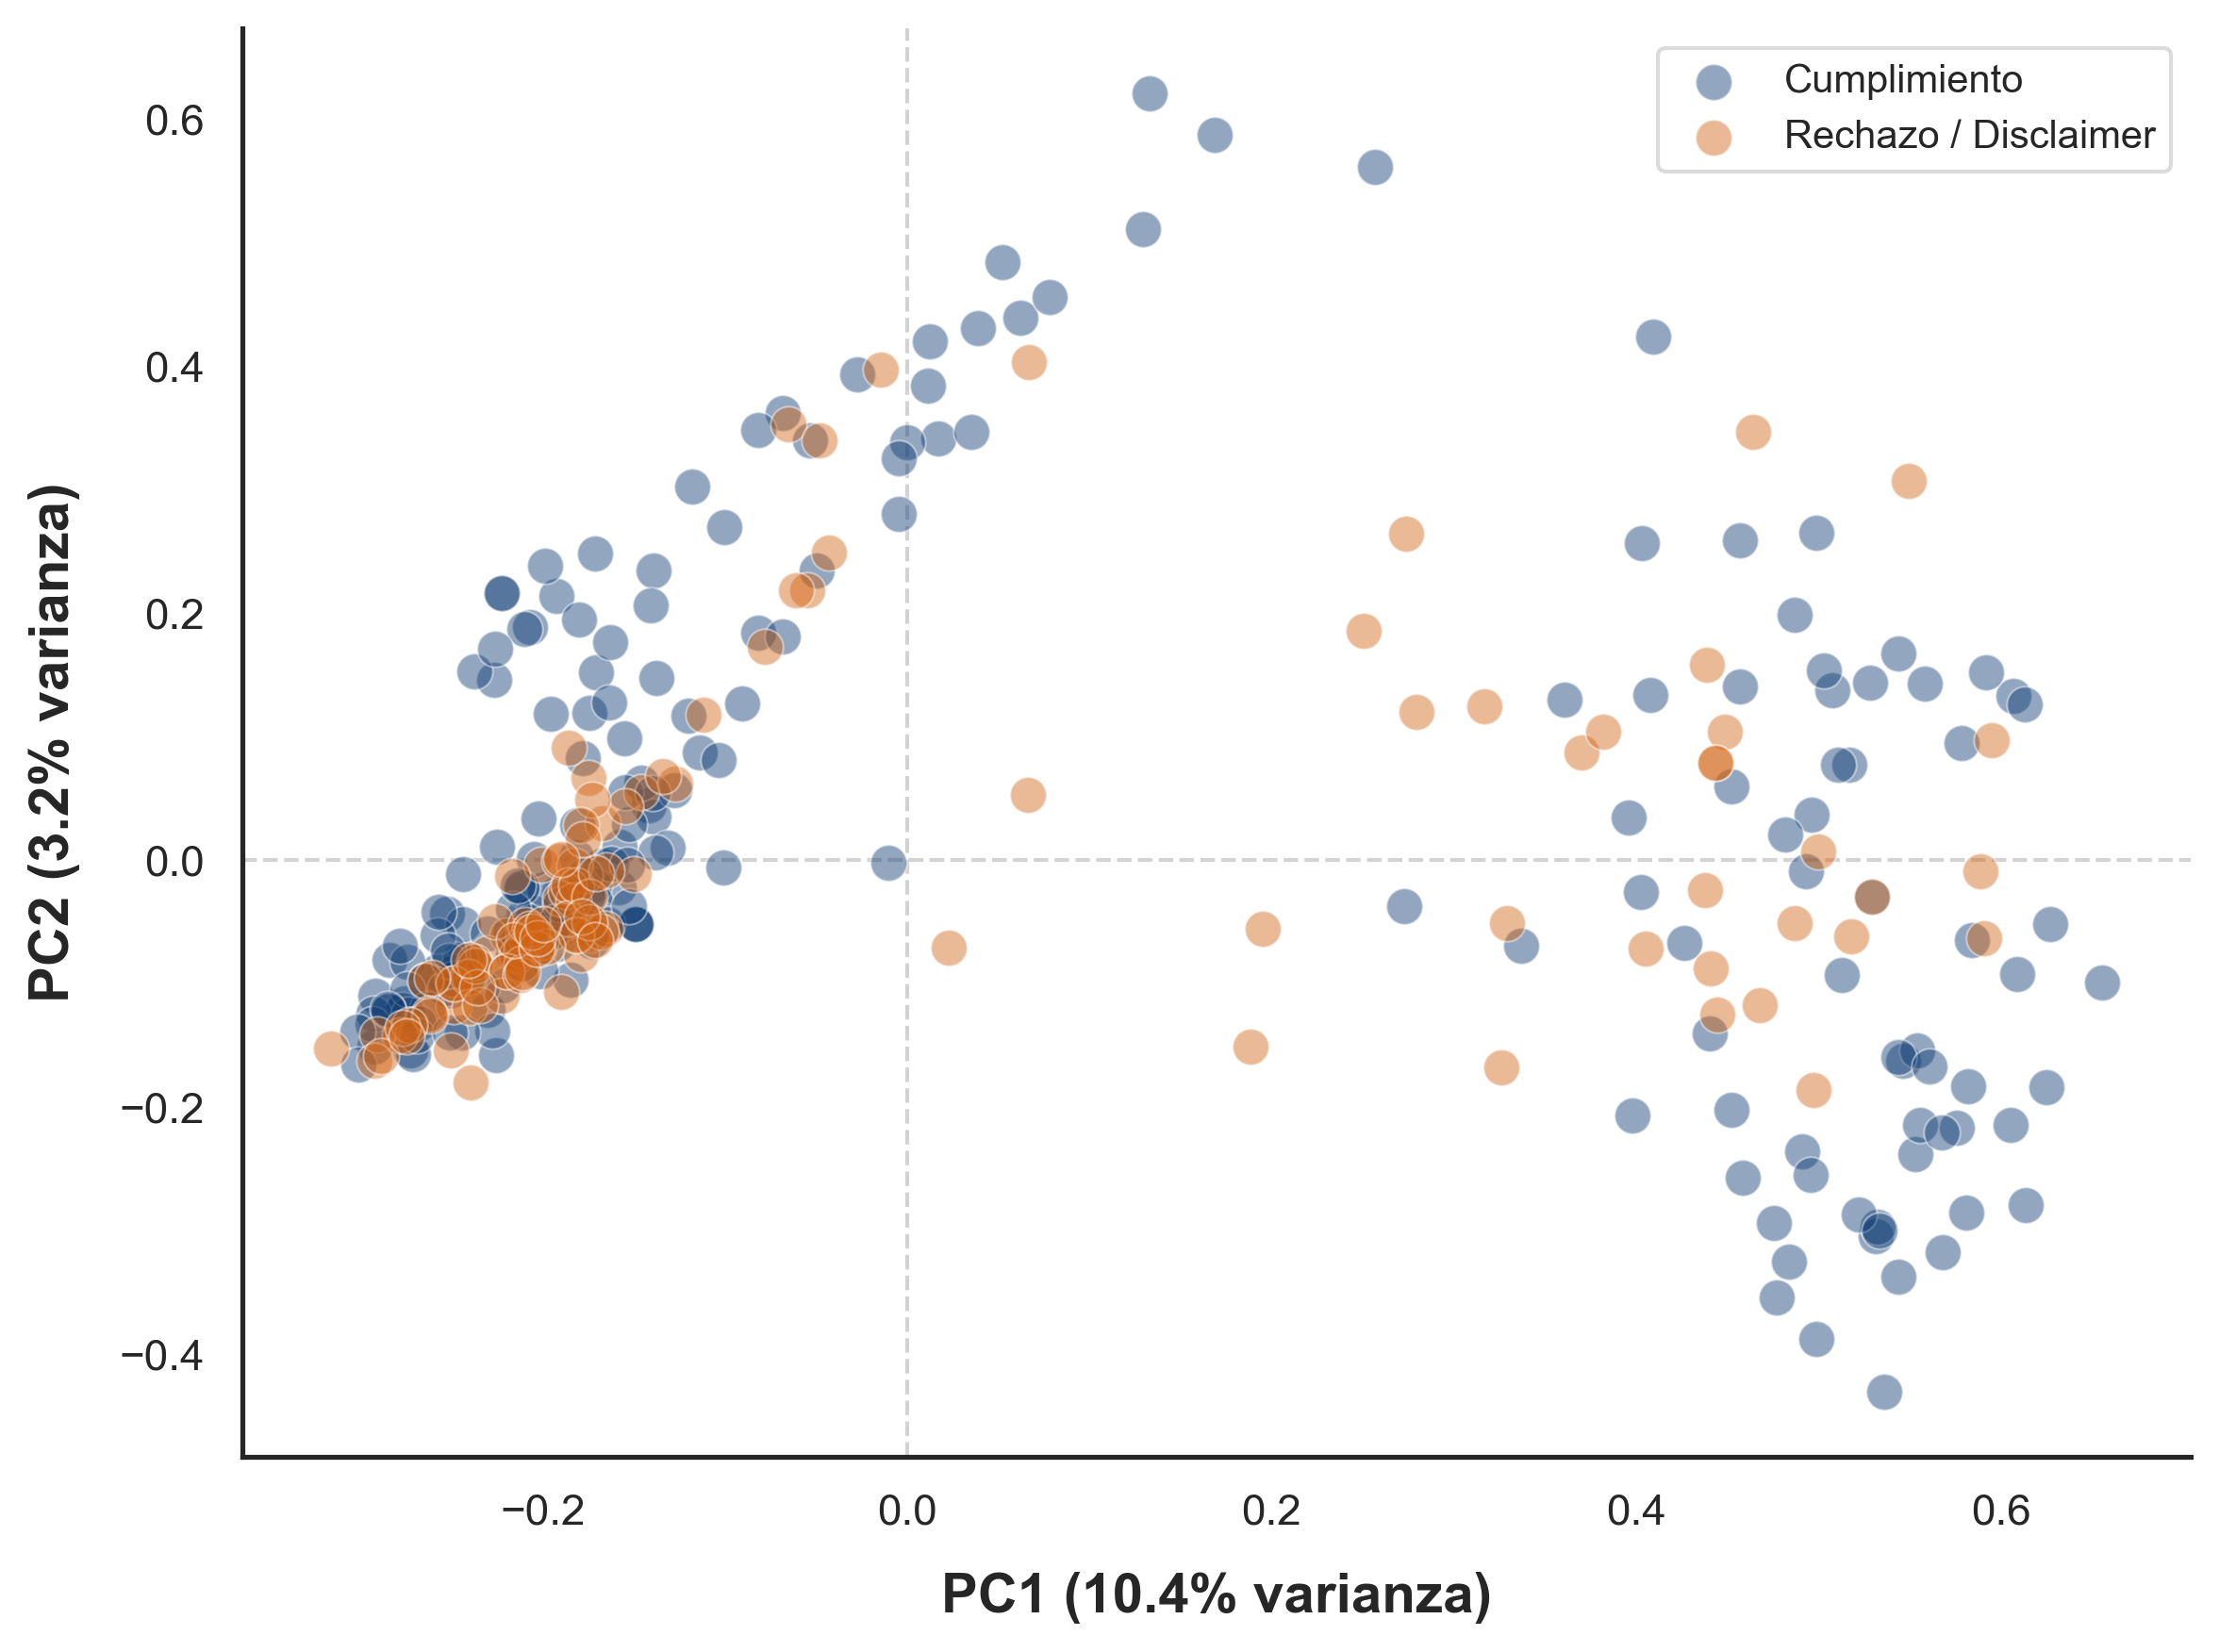
\includegraphics[width=0.48\textwidth]{pca-plot.png}
\caption{Visualización bidimensional del conjunto de datos ShareChat balanceado mediante reducción de dimensionalidad PCA ($d=1000 \rightarrow 2$).}
\label{fig:pca_plot}
\end{figure}

Para analizar el comportamiento de los modelos frente a diferentes cantidades de datos, medimos los tiempos de ejecución tomando subconjuntos cada vez más grandes del dataset de entrenamiento.

\subsection{Análisis del Comportamiento de KNN}
Como podemos ver en la Figura \ref{fig:complexity_knn}, el tiempo de predicción de nuestra implementación manual de KNN crece de manera totalmente lineal a medida que aumentamos el tamaño de los datos de entrenamiento $N$. Esto coincide con nuestra estimación teórica de $\mathcal{O}(M \cdot N \cdot d)$. Debido a que programamos el código directamente en Python interpretado y trabajamos con vectores grandes ($d=1000$), calcular repetidamente similitudes coseno de forma manual se vuelve extremadamente lento y costoso para la computadora.

\begin{figure}[htbp]
\centering
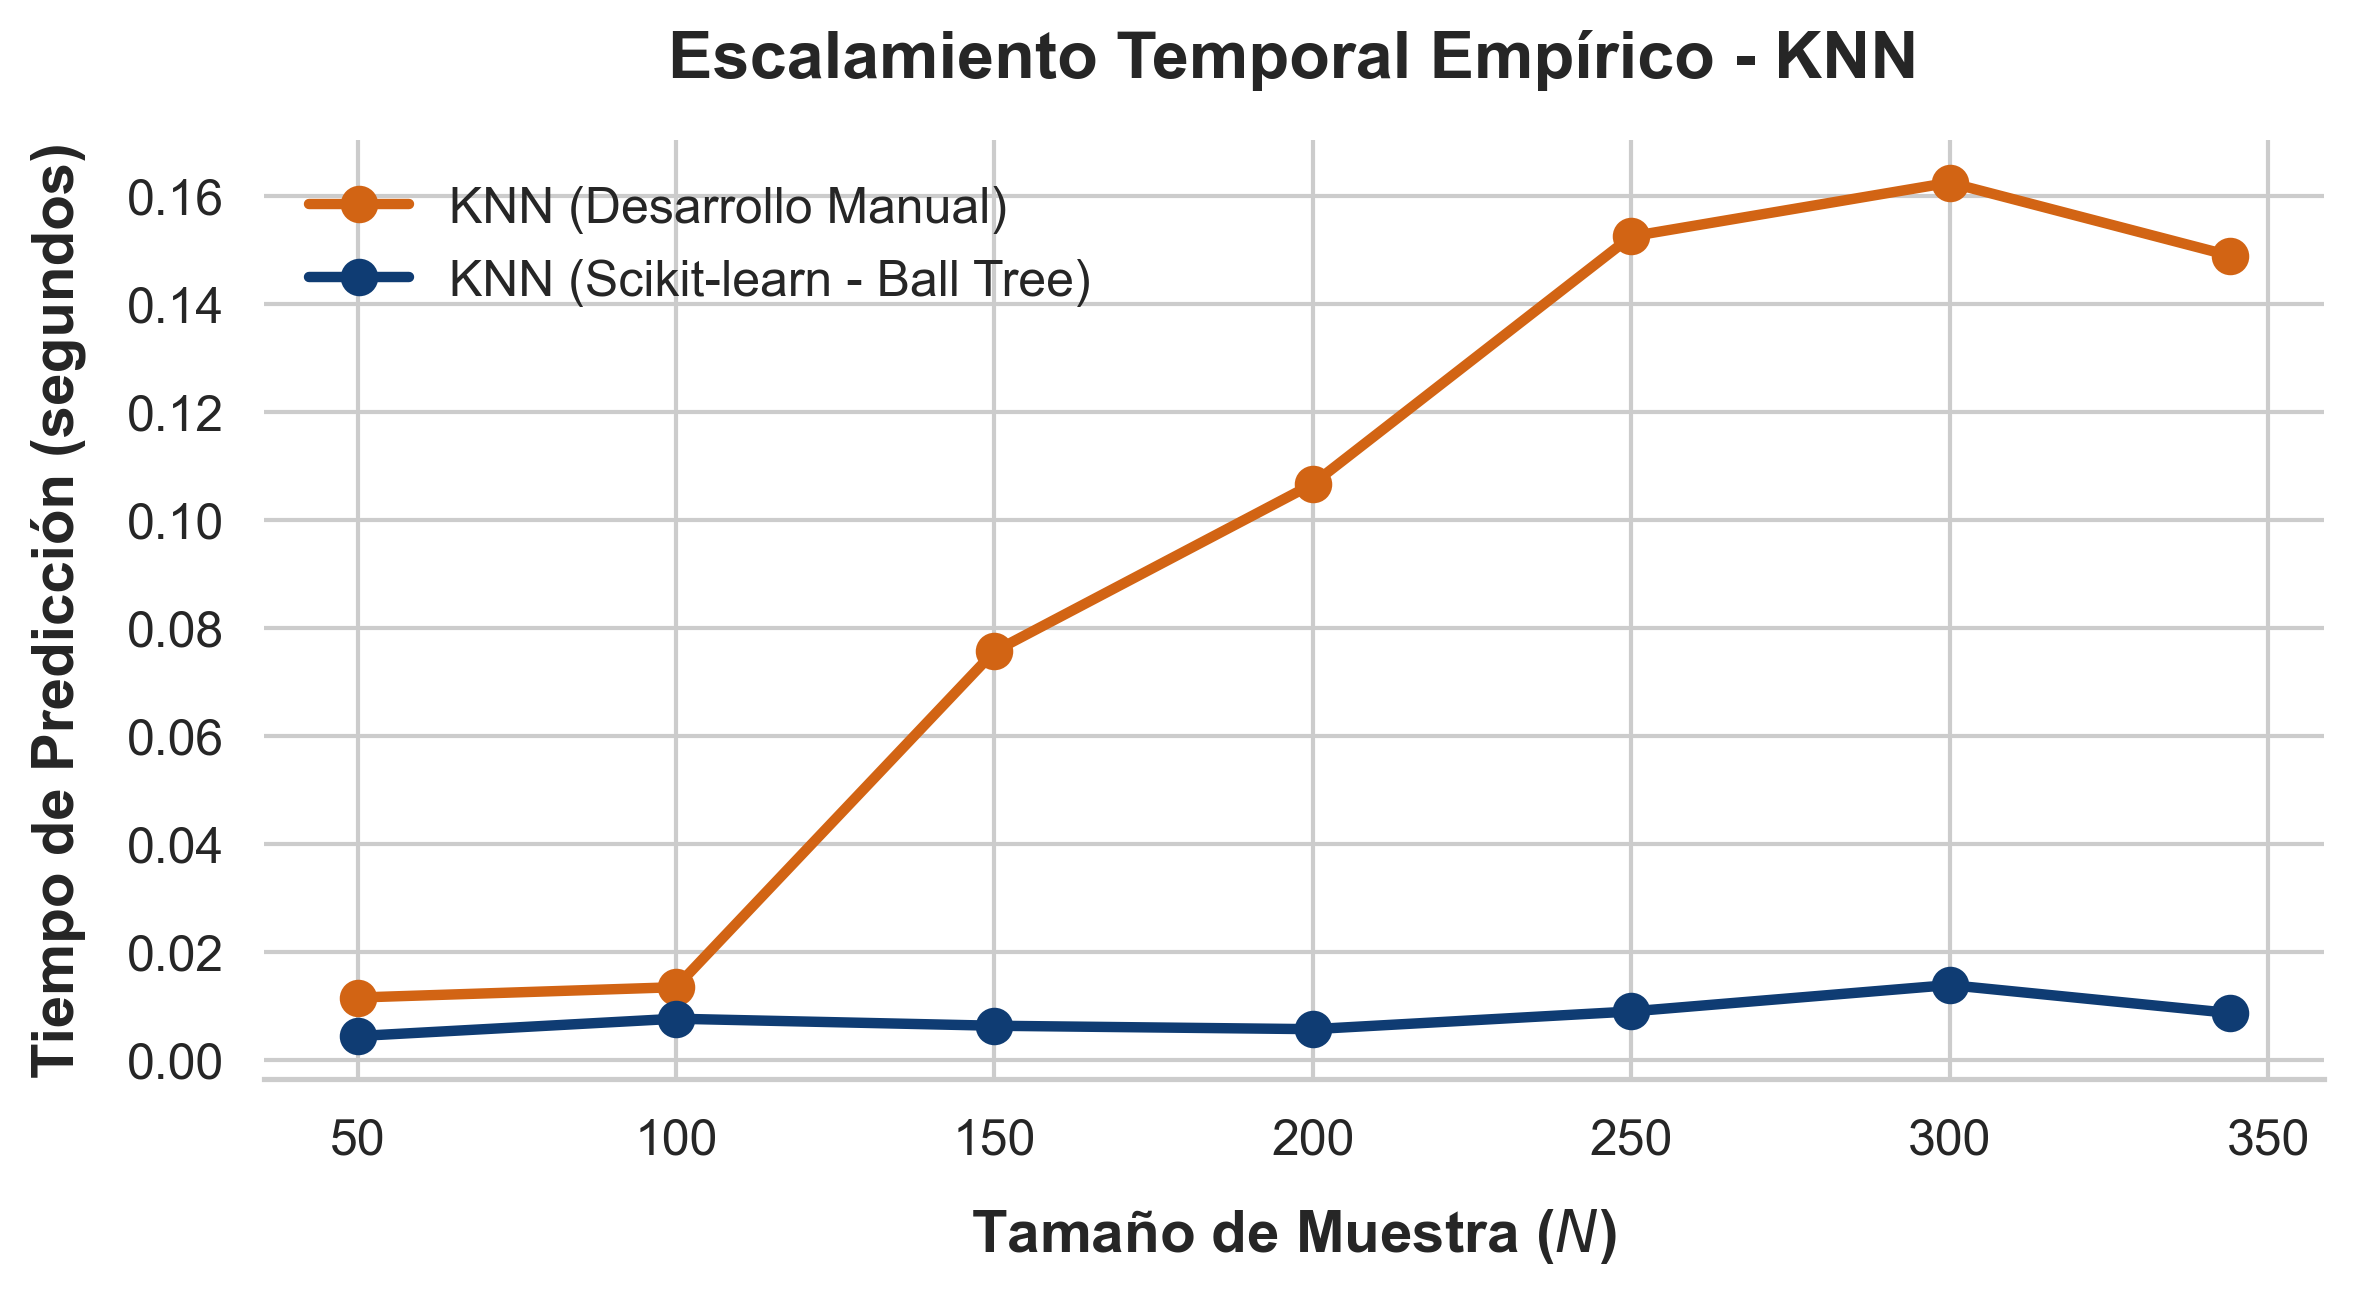
\includegraphics[width=0.48\textwidth]{complexity-knn.png}
\caption{Escalamiento temporal empírico en la predicción de KNN ($K=5, d=1000$): Implementación manual frente a scikit-learn.}
\label{fig:complexity_knn}
\end{figure}

Por el contrario, el modelo de la librería \texttt{scikit-learn} (\texttt{KNeighborsClassifier}) es mucho más rápido porque realiza estos cálculos en segundo plano con librerías optimizadas en lenguajes compilados (como C) usando operaciones matriciales avanzadas. Además, \texttt{scikit-learn} puede utilizar un \textbf{KD-Tree} para acelerar las búsquedas:
\begin{itemize}
    \item \textbf{KD-Tree}: Esta estructura organiza los datos dividiendo el espacio. Construirlo toma un tiempo de entrenamiento de $\mathcal{O}(N \cdot d \log N)$, pero a cambio permite buscar los vecinos más cercanos en un tiempo promedio de $\mathcal{O}(d \log N)$ por cada consulta.
    \item \textbf{Maldición de la Dimensionalidad}: Aunque los KD-Trees son muy útiles en dimensiones bajas, la teoría \cite{knuth1976} y los resultados de nuestras pruebas demuestran que cuando trabajamos con muchas dimensiones (como nuestras $d=1000$ características de texto), el espacio es tan grande que el árbol pierde eficiencia. En estos casos, el algoritmo se ve obligado a revisar casi todos los caminos, por lo que su complejidad vuelve a ser lineal, similar a la búsqueda manual. A pesar de esto, la versión de \texttt{scikit-learn} sigue siendo órdenes de magnitud más rápida gracias a su optimización interna a nivel de hardware.
\end{itemize}

\subsection{Análisis del Comportamiento de Regresión Logística}
En el caso de la Regresión Logística manual, entrenar con descenso de gradiente ordinario tiene un costo lineal de $\mathcal{O}(T \cdot N \cdot d)$. Para que los pesos alcancen valores estables y el costo deje de disminuir, necesitamos realizar muchas iteraciones de entrenamiento ($T \ge 2000$), lo cual hace que el tiempo de ejecución aumente rápidamente a medida que agregamos más ejemplos de entrenamiento $N$ (ver Figura \ref{fig:complexity_rl}).

\begin{figure}[htbp]
\centering
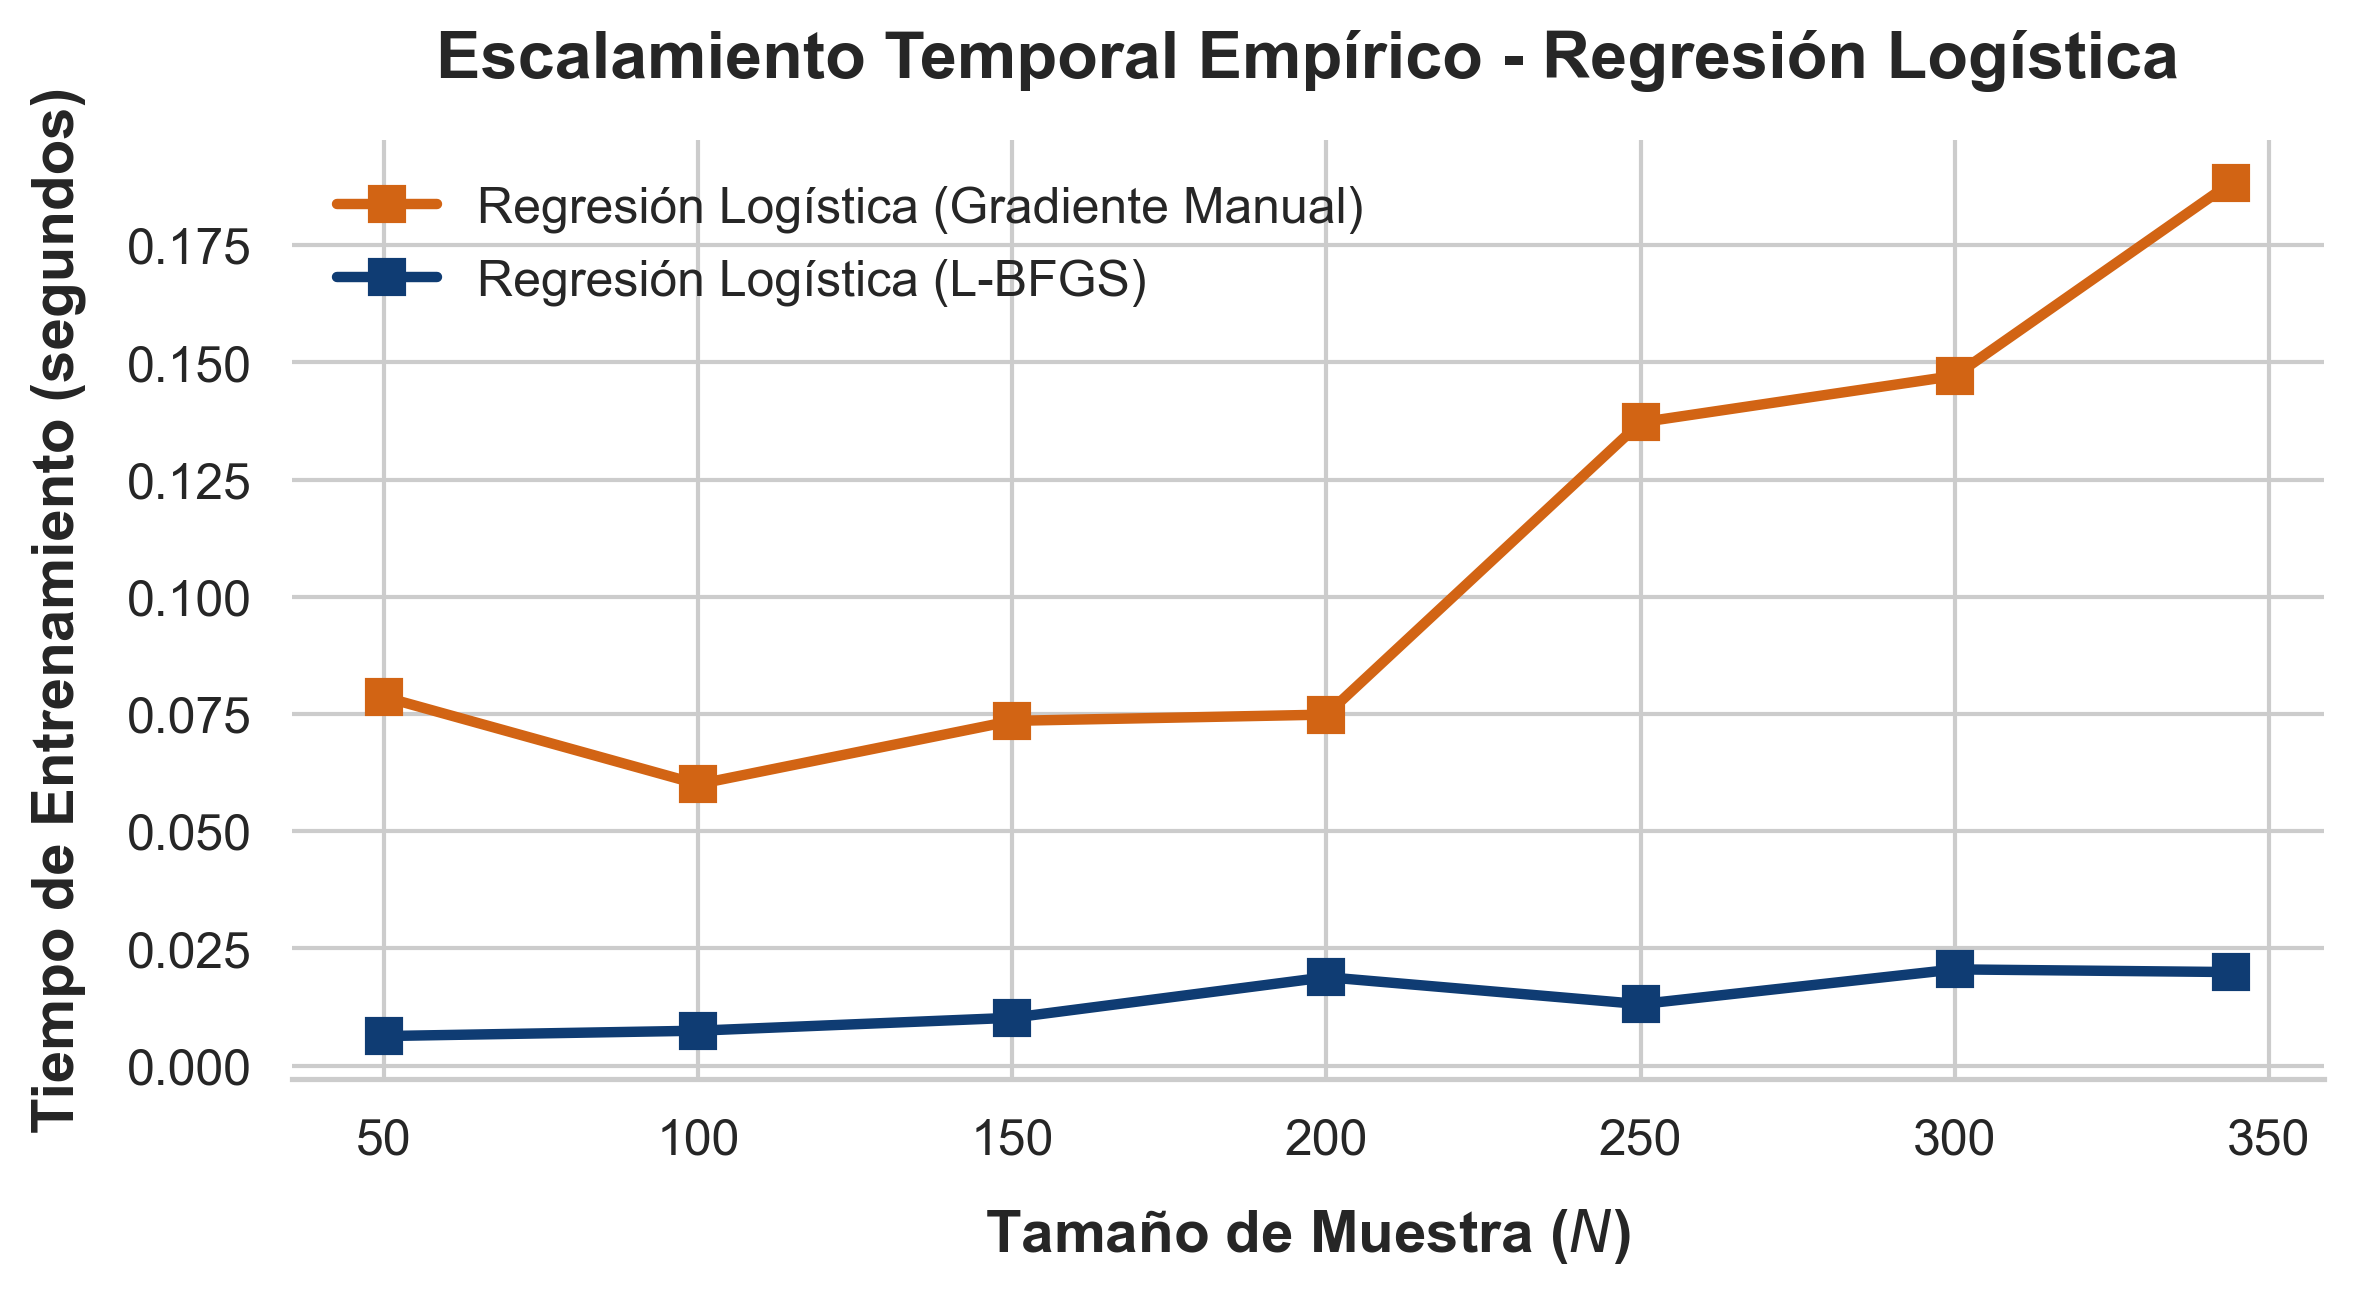
\includegraphics[width=0.48\textwidth]{complexity-rl.png}
\caption{Escalamiento temporal empírico en el entrenamiento de Regresión Logística ($T=2000, d=1000$): GD manual frente a L-BFGS.}
\label{fig:complexity_rl}
\end{figure}

Por su parte, \texttt{scikit-learn} (\texttt{LogisticRegression}) resuelve esto utilizando un optimizador muy eficiente llamado \textbf{L-BFGS} (un método de segundo orden) \cite{nocedal2006}:
\begin{itemize}
    \item \textbf{Uso de Curvatura de Segundo Orden}: Mientras que nuestro descenso de gradiente manual solo mira la dirección de la pendiente más inclinada (primer orden), el optimizador L-BFGS estima la curvatura de la función (segundas derivadas). Esto le permite dar pasos de ajuste mucho más precisos e inteligentes.
    \item \textbf{Velocidad de Convergencia}: Al usar la información de curvatura, L-BFGS logra encontrar el valor óptimo en muy pocas iteraciones ($T' \ll T$), reduciendo enormemente el tiempo de entrenamiento. En la práctica, el costo de este solver es de aproximadamente $\mathcal{O}(T' \cdot m \cdot d)$, donde $m$ (historial de memoria) es un valor pequeño. En la Figura \ref{fig:complexity_rl} observamos cómo la curva de \texttt{scikit-learn} se mantiene casi plana e instantánea, mostrando una enorme ventaja sobre la versión hecha a mano.
\end{itemize}

\section{Conclusión}
El análisis de la complejidad computacional demuestra la gran importancia de diseñar y utilizar algoritmos eficientes en problemas prácticos de seguridad en Inteligencia Artificial. Escribir los algoritmos manuales en este proyecto nos ha permitido comprender en detalle las matemáticas detrás de KNN y de la Regresión Logística. Sin embargo, para trabajar con datos del mundo real, estas versiones manuales no son viables en producción debido al alto tiempo que toma calcular distancias en altas dimensiones de forma repetida o por la gran cantidad de iteraciones que necesita el descenso de gradiente estándar.

Las técnicas de optimización que usan las librerías profesionales de código abierto, como la vectorización de bajo nivel, los árboles de búsqueda espacial y los optimizadores avanzados de segundo orden, son fundamentales para que los sistemas de análisis y clasificación sobre prompts de LLMs sean rápidos y utilizables en la práctica.

\begin{thebibliography}{6}

\bibitem{hastie2009}
Hastie, T., Tibshirani, R., \& Friedman, J. (2009). \emph{The Elements of Statistical Learning: Data Mining, Inference, and Prediction} (2nd ed.). Springer.

\bibitem{tucnguyen2024}
Nguyen, T. (2024). \emph{ShareChat: A large-scale dataset of multi-turn conversations with LLMs} (Technical Report). Hugging Face. \url{https://huggingface.co/datasets/tucnguyen/ShareChat}

\bibitem{pedregosa2011}
Pedregosa, F., Varoquaux, G., Gramfort, A., Michel, V., Thirion, B., Grisel, O., Blondel, M., Prettenhofer, P., Weiss, R., Dubourg, V., Vanderplas, J., Passos, A., Cournapeau, D., Brucher, M., Perrot, M., \& Duchesnay, E. (2011). Scikit-learn: Machine learning in Python. \emph{Journal of Machine Learning Research}, \emph{12}, 2825--2830.

\bibitem{nocedal2006}
Nocedal, J., \& Wright, S. J. (2006). \emph{Numerical optimization} (2nd ed.). Springer.

\bibitem{knuth1976}
Knuth, D. E. (1976). Big omicron and big omega and big theta. \emph{ACM SIGACT News}, \emph{8}(2), 18--24.

\bibitem{ouyang2022}
Ouyang, L., Wu, J., Jiang, X., Almeida, D., Wainwright, C. L., Mishkin, P., ... \& Lowe, R. (2022). Training language models to follow instructions with human feedback. \emph{Advances in Neural Information Processing Systems}, \emph{35}, 27730--27744.

\end{thebibliography}

\end{document}
